\documentclass[12pt,a4paper]{article}
\usepackage[utf8]{inputenc}
\usepackage[turkish]{babel}
\usepackage{amsmath,amssymb,amsfonts,amsthm}
\usepackage{geometry}
\geometry{top=2.5cm,bottom=2.5cm,left=2.5cm,right=2.5cm}
\usepackage{xcolor}
\usepackage{tikz}
\usetikzlibrary{babel,arrows.meta,positioning,calc}
\usepackage{pgfplots}
\pgfplotsset{compat=1.18}
\usepackage[most]{tcolorbox}
\usepackage{hyperref}
\usepackage{caption}
\usepackage{booktabs}
\usepackage{tabularx}

% Renk Tanımlamaları ve Kutular
\definecolor{mainblue}{RGB}{26, 82, 118}
\definecolor{alertred}{RGB}{180, 40, 40}
\definecolor{okgreen}{RGB}{34, 139, 34}
\definecolor{boxbg}{RGB}{245, 247, 250}
\definecolor{tealblue}{RGB}{0, 120, 130}
\definecolor{purp}{RGB}{128, 0, 128}

\tcbset{
  commonbox/.style={
    arc=2mm,
    breakable,
    enhanced,
    boxrule=1pt,
    left=4mm, right=4mm, top=3mm, bottom=3mm
  }
}

\newtcolorbox{uyari}[1][]{
  commonbox,
  colback=red!5!white,
  colframe=alertred,
  fonttitle=\bfseries,
  title={Düzeltme / Dikkat Edilmesi Gereken Hata},
  #1
}

\newtcolorbox{ornek}[2][]{
  commonbox,
  colback=mainblue!5!white,
  colframe=mainblue,
  fonttitle=\bfseries,
  title={Örnek: #2},
  #1
}

\newtcolorbox{odev}[2][]{
  commonbox,
  colback=okgreen!5!white,
  colframe=okgreen,
  fonttitle=\bfseries,
  title={Ödev ve Çözümü: #2},
  #1
}

\newtcolorbox{tanim}[2][]{
  commonbox,
  colback=gray!5!white,
  colframe=gray!60!black,
  fonttitle=\bfseries,
  title={Tanım: #2},
  #1
}

\newtcolorbox{sezgi}[2][]{
  commonbox,
  colback=tealblue!5!white,
  colframe=tealblue,
  fonttitle=\bfseries,
  title={Sezgisel Bakış ve Basit Anlatım: #2},
  #1
}

\newtcolorbox{teorem}[2][]{
  commonbox,
  colback=purp!5!white,
  colframe=purp,
  fonttitle=\bfseries,
  title={Teorem: #2},
  #1
}

\title{\textbf{İSTATİSTİK TEORİSİ}\\[0.3em] \Large 1. Hafta: Momentler, MÇF, Temel Eşitsizlikler ve Gamma Fonksiyonu}
\author{Kapsamlı Konu Anlatımı, Matematiksel İspatlar, Sezgisel Analizler ve Çözümlü Problemler}
\date{}

\begin{document}

\maketitle

\begin{abstract}
Bu çalışma; İstatistik Teorisi dersinin 1. haftasında yer alan \textbf{Moment Kavramı (Orijine ve Ortalamaya Göre Momentler)}, \textbf{Çarpıklık ve Basıklık}, \textbf{Markov, Chebyshev ve Jensen Eşitsizlikleri}, \textbf{Moment Çıkaran Fonksiyon (MÇF)}, \textbf{Bağımsız Toplamlar ve Teklik Teoremi}, \textbf{Euler Gamma Fonksiyonu} ve $\Gamma(1/2) = \sqrt{\pi}$ ispatını içermektedir. Ağır matematiksel integrallerin yanında her kavramın arkasındaki sezgisel mantık, el yazısı ders notlarındaki kritik işlem hatalarının düzeltmeleri, vektörel TikZ grafikleri ve adım adım sınav tipi çözümlerle desteklenmiştir.
\end{abstract}

\hrule
\vspace{1em}

\section{Giriş ve Moment Kavramı}

\begin{sezgi}{Moment Nedir ve Neden İhtiyaç Duyarız?}
Bir olasılık dağılımı ($f(x)$) elimizde sonsuz sayıda noktadan oluşan karmaşık bir eğri veya veri yığını olarak bulunur. Bu eğrinin tüm geometrik ve istatistiksel karakterini birkaç kritik sayı ile özetlemek isteriz:
\begin{itemize}
    \item \textbf{1. Moment ($\mu$ - Ortalama):} Dağılımın sayı doğrusundaki \textbf{ağırlık merkezidir}. Eğri homojen ağırlıklı bir tahterevalli olsaydı, parmağımızı tam nereye koyarsak dengede kalırdı? İşte bu denge noktası $E(X)$'tir.
    \item \textbf{2. Merkezsel Moment ($\sigma^2$ - Varyans):} Verilerin bu ağırlık merkezinden ne kadar uzağa saçıldığını, yani \textbf{belirsizliğin ve riskin büyüklüğünü} ölçer.
    \item \textbf{3. Moment (Çarpıklık / Skewness):} Dağılımın simetrisini inceler. Kuyruk sağa doğru mu uzanıyor (pozitif çarpık), yoksa sola doğru mu (negatif çarpık)?
    \item \textbf{4. Moment (Basıklık / Kurtosis):} Dağılımın tepe noktasının sivriliğini ve kuyrukların kalınlığını (uç değer riskini / black swan olaylarını) ölçer.
\end{itemize}
Kısacası momentler, bir olasılık dağılımının boyunu, kilosunu ve karakteristik hatlarını belirleyen \textbf{biyometrik kimlik kartıdır}.
\end{sezgi}

\begin{tanim}{Moment Tanımları}
Bir $X$ rastgele değişkeni için:
\begin{enumerate}
    \item \textbf{Orijine Göre $k$. Moment ($k$. Ham / Merkezsel Olmayan Moment - Raw Moment):}
    \begin{equation}
        \mu'_k = E(X^k) = 
        \begin{cases}
            \sum_x x^k P(X = x), & \text{kesikli durumda} \\[0.5em]
            \int_{-\infty}^{\infty} x^k f(x) \, dx, & \text{sürekli durumda}
        \end{cases}
    \end{equation}
    Özel olarak $k=1$ için 1. ham moment kitle ortalamasını ($\mu$) verir:
    \begin{equation}
        \mu'_1 = E(X) = \mu
    \end{equation}

    \item \textbf{$k$. Merkezsel Moment (Central Moment):}
    Ortalama ($\mu$) etrafındaki sapmaların kuvvetlerinin beklenen değeridir:
    \begin{equation}
        \mu_k = E\left[(X - \mu)^k\right] = 
        \begin{cases}
            \sum_x (x - \mu)^k P(X = x), & \text{kesikli durumda} \\[0.5em]
            \int_{-\infty}^{\infty} (x - \mu)^k f(x) \, dx, & \text{sürekli durumda}
        \end{cases}
    \end{equation}
    Özel olarak:
    \begin{itemize}
        \item $k=1$ için: $\mu_1 = E[X - \mu] = E(X) - \mu = 0$ (Ortalamadan sapmaların beklenen değeri daima sıfırdır).
        \item $k=2$ için: $\mu_2 = E\left[(X - \mu)^2\right] = V(X) = \sigma^2$ (Varyans).
    \end{itemize}
\end{enumerate}
\end{tanim}

\subsection{Merkezsel Momentler ile Ham Momentler Arasındaki Cebirsel İlişki}
Binom açılımı $(X - \mu)^k = \sum_{j=0}^k \binom{k}{j} X^j (-\mu)^{k-j}$ kullanılarak merkezsel momentler ham momentler cinsinden yazılabilir:
\begin{align}
    \mu_2 &= E\left[(X - \mu)^2\right] = E(X^2 - 2\mu X + \mu^2) = E(X^2) - 2\mu E(X) + \mu^2 = \mu'_2 - (\mu'_1)^2 \\
    \mu_3 &= E\left[(X - \mu)^3\right] = \mu'_3 - 3\mu'_2 \mu'_1 + 2(\mu'_1)^3 \\
    \mu_4 &= E\left[(X - \mu)^4\right] = \mu'_4 - 4\mu'_3 \mu'_1 + 6\mu'_2 (\mu'_1)^2 - 3(\mu'_1)^4
\end{align}

\subsection{Standartlaştırılmış Momentler: Çarpıklık ve Basıklık}
\begin{itemize}
    \item \textbf{Çarpıklık Katsayısı (Skewness - $\alpha_3$):}
    \begin{equation}
        \alpha_3 = \frac{\mu_3}{\sigma^3} = \frac{E\left[(X - \mu)^3\right]}{\sigma^3}
    \end{equation}
    $\alpha_3 = 0$ ise dağılım simetriktir (örn: Normal dağılım). $\alpha_3 > 0$ ise sağa uzun kuyruklu (pozitif çarpık), $\alpha_3 < 0$ ise sola uzun kuyrukludur (negatif çarpık).

    \item \textbf{Basıklık Katsayısı (Kurtosis - $\alpha_4$):}
    \begin{equation}
        \alpha_4 = \frac{\mu_4}{\sigma^4} = \frac{E\left[(X - \mu)^4\right]}{\sigma^4}
    \end{equation}
    Standart normal dağılım için $\alpha_4 = 3$'tür. Bu nedenle fazlalık basıklık (excess kurtosis) $\gamma_2 = \alpha_4 - 3$ olarak tanımlanır. $\alpha_4 > 3$ ise sivri ve kalın kuyruklu (leptokurtik), $\alpha_4 < 3$ ise basık ve ince kuyrukludur (platikurtik).
\end{itemize}

\begin{ornek}{Normal Dağılımın Ortalamasının Doğrudan İntegralle Hesaplanması}
$X \sim N(\mu, \sigma^2)$ dağılımına sahip sürekli bir rastgele değişkenin olasılık yoğunluk fonksiyonu:
\begin{equation}
    f(x) = \frac{1}{\sqrt{2\pi\sigma^2}} \exp\left(-\frac{1}{2}\left(\frac{x - \mu}{\sigma}\right)^2\right), \quad -\infty < x < \infty
\end{equation}
şeklindedir. $E(X)$ beklenen değerini doğrudan integral tanımıyla hesaplayınız.

\bigskip
\textbf{Çözüm Adımları:}
\begin{enumerate}
    \item Beklenen değer tanımını yazalım:
    \begin{equation}
        E(X) = \int_{-\infty}^{\infty} x f(x) \, dx = \frac{1}{\sqrt{2\pi\sigma^2}} \int_{-\infty}^{\infty} x \, e^{-\frac{1}{2}\left(\frac{x - \mu}{\sigma}\right)^2} dx
    \end{equation}
    \item Standartlaştırma ($z$-dönüşümü) uygulayalım:
    \begin{equation}
        z = \frac{x - \mu}{\sigma} \implies x = \sigma z + \mu \implies dx = \sigma \, dz
    \end{equation}
    \item Bu değişken dönüşümünü integrale yerleştirelim ($\sqrt{\sigma^2} = \sigma$ çarpanı diferansiyeldeki $\sigma$ ile tam sadeleşir):
    \begin{align}
        E(X) &= \frac{1}{\sqrt{2\pi}\sigma} \int_{-\infty}^{\infty} (\sigma z + \mu) \, e^{-\frac{1}{2}z^2} (\sigma \, dz) \notag \\
        &= \underbrace{\frac{\sigma}{\sqrt{2\pi}} \int_{-\infty}^{\infty} z \, e^{-\frac{1}{2}z^2} dz}_{I_1} + \underbrace{\mu \int_{-\infty}^{\infty} \frac{1}{\sqrt{2\pi}} e^{-\frac{1}{2}z^2} dz}_{I_2}
    \end{align}

    \item \textbf{$I_2$ İntegralinin Hesabı:}  
    Standart normal yoğunluk fonksiyonunun ($N(0,1)$) tüm reel eksendeki toplam alanı olasılık aksiyomları gereği 1'dir:
    \begin{equation}
        \int_{-\infty}^{\infty} \frac{1}{\sqrt{2\pi}} e^{-\frac{1}{2}z^2} dz = 1 \implies I_2 = \mu \cdot 1 = \mu
    \end{equation}

    \item \textbf{$I_1$ İntegrali ve Tek Fonksiyon Püf Noktası:}  
    $g(z) = z \, e^{-\frac{1}{2}z^2}$ fonksiyonunda $z$ yerine $-z$ yazalım:
    \begin{equation}
        g(-z) = (-z) e^{-\frac{1}{2}(-z)^2} = -z e^{-\frac{1}{2}z^2} = -g(z)
    \end{equation}
    $g(z)$ bir \textbf{tek (odd) fonksiyondur}. Simetrik $[-\infty, \infty]$ aralığında mutlak integrallenebilir bir tek fonksiyonun negatif taraftaki alanı ile pozitif taraftaki alanı birbirini tam olarak sıfırlar:
    \begin{equation}
        I_1 = \frac{\sigma}{\sqrt{2\pi}} \int_{-\infty}^{\infty} z e^{-\frac{1}{2}z^2} dz = 0
    \end{equation}
\end{enumerate}
Sonuç olarak:
\begin{equation}
    E(X) = I_1 + I_2 = 0 + \mu = \mu
\end{equation}
bulunur.
\end{ornek}

\begin{uyari}
\textbf{El Yazısı Notlardaki Yaklaşım ve Matematiksel Düzeltme:}
\begin{itemize}
    \item 2. sayfadaki el yazısı notlarda $I_1$ integrali için $u = z^2$ dönüşümü yapılarak integral $(-\infty, 0)$ ve $(0, \infty)$ aralıklarına bölünmeye çalışılmıştır.
    \item Ancak $z < 0$ iken $u = z^2 \implies z = -\sqrt{u}$ olduğundan diferansiyel adımı işaret karmaşasına yol açmaktadır.
    \item Sonuç $-\frac{\sigma}{\sqrt{2\pi}} + \frac{\sigma}{\sqrt{2\pi}} = 0$ olarak doğru tamamlansa da; $z e^{-z^2/2}$ integrandı tek fonksiyon olduğundan simetriden dolayı doğrudan $I_1 = 0$ yazmak hem matematiksel açıdan en şık hem de sınav puanlama standartlarında en risksiz yöntemdir.
\end{itemize}
\end{uyari}

\begin{center}
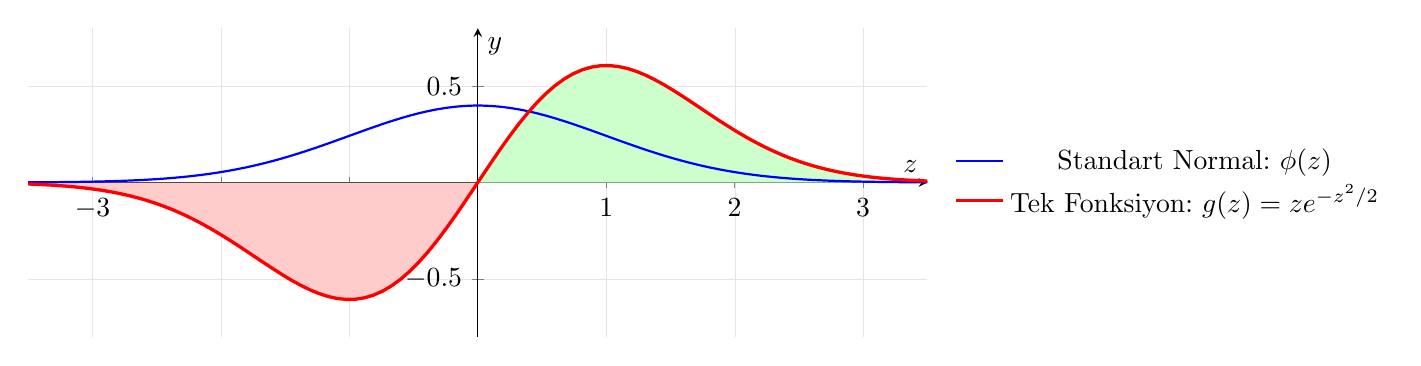
\begin{tikzpicture}
\begin{axis}[
    width=13cm, height=5.5cm,
    axis lines=center,
    xlabel={$z$}, ylabel={$y$},
    xmin=-3.5, xmax=3.5,
    ymin=-0.8, ymax=0.8,
    samples=100,
    domain=-3.5:3.5,
    grid=both,
    grid style={line width=.1pt, draw=gray!20},
    legend style={
        at={(1.02,0.5)},
        anchor=west,
        draw=none
    }
]
    % Sol alan tarama (negatif alan)
    \addplot[fill=red!20, draw=none, domain=-3.5:0, forget plot] {x * exp(-x^2/2)} \closedcycle;
    % Sağ alan tarama (pozitif alan)
    \addplot[fill=green!20, draw=none, domain=0:3.5, forget plot] {x * exp(-x^2/2)} \closedcycle;

    % Standart normal
    \addplot[blue, thick] {1/sqrt(2*pi)*exp(-x^2/2)};
    \addlegendentry{Standart Normal: $\phi(z)$}

    % z * exp(-z^2/2) tek fonksiyon
    \addplot[red, very thick] {x * exp(-x^2/2)};
    \addlegendentry{Tek Fonksiyon: $g(z) = z e^{-z^2/2}$}
\end{axis}
\end{tikzpicture}
\captionof{figure}{Tek Fonksiyon Özelliği: Kırmızı eğri $g(-z) = -g(z)$ simetrisine sahiptir. Negatif bölgedeki alan (kırmızı taralı) ile pozitif bölgedeki alan (yeşil taralı) eşit büyüklükte ve zıt işaretli olduğundan integral net sıfır verir.}
\end{center}

---

\section{Olasılık Teorisinde Temel Eşitsizlikler}

Momentler dağılım hakkında genel sınırlar çizmemize olanak tanır. Dağılımın tam fonksiyonel formunu bilmesek dahi sadece ortalama ve varyans bilgisiyle olasılık sınırları hesaplayabiliriz.

\subsection{1. Markov Eşitsizliği}
\begin{teorem}{Markov Eşitsizliği}
$X$ negatif değer almayan ($X \ge 0$) bir rastgele değişken ve $a > 0$ herhangi bir pozitif reel sayı olsun. Bu durumda:
\begin{equation}
    P(X \ge a) \le \frac{E(X)}{a}
\end{equation}
\end{teorem}

\begin{sezgi}{Markov Eşitsizliğinin Anlamı}
"Bir şirkette çalışanların maaş ortalaması 20.000 TL ise, çalışanların en fazla kaçta kaçı 100.000 TL veya üzerinde kazanıyor olabilir?"  
Markov kuralına göre: $P(X \ge 100.000) \le \frac{20.000}{100.000} = \frac{1}{5} = \%20$.  
Eğer çalışanların \%20'sinden fazlası 100.000 TL alsaydı, sadece onların getireceği pay bile ortalamayı 20.000 TL'nin üzerine fırlatırdı! Dağılım ne olursa olsun bu sınır aşılamaz.
\end{sezgi}

\textbf{Matematiksel İspat:}
$X \ge 0$ sürekli bir değişken olsun (kesikli durum tamamen paraleldir):
\begin{align}
    E(X) &= \int_0^\infty x f(x) \, dx = \int_0^a x f(x) \, dx + \int_a^\infty x f(x) \, dx \notag \\
    &\ge \int_a^\infty x f(x) \, dx \quad (\text{çünkü } x \ge 0 \text{ ve } f(x) \ge 0 \text{ olduğundan } \int_0^a \ge 0) \notag \\
    &\ge \int_a^\infty a f(x) \, dx \quad (\text{çünkü integral bölgesinde } x \ge a) \notag \\
    &= a \int_a^\infty f(x) \, dx = a P(X \ge a)
\end{align}
Her iki taraf $a > 0$'a bölündüğünde $P(X \ge a) \le \frac{E(X)}{a}$ elde edilir. $\blacksquare$

\subsection{2. Chebyshev Eşitsizliği}
\begin{teorem}{Chebyshev Eşitsizliği}
Ortalaması $\mu$ ve sonlu varyansı $\sigma^2$ olan herhangi bir $X$ rastgele değişkeni için, her $k > 0$ veya her $\epsilon > 0$ için:
\begin{equation}
    P(|X - \mu| \ge k\sigma) \le \frac{1}{k^2} \quad \iff \quad P(|X - \mu| < k\sigma) \ge 1 - \frac{1}{k^2}
\end{equation}
Benzer şekilde $\epsilon = k\sigma$ alınırsa:
\begin{equation}
    P(|X - \mu| \ge \epsilon) \le \frac{\sigma^2}{\epsilon^2}
\end{equation}
\end{teorem}

\textbf{Matematiksel İspat:}
$Y = (X - \mu)^2$ rastgele değişkenini tanımlayalım. $Y \ge 0$'dır ve $E(Y) = E[(X-\mu)^2] = \sigma^2$'dir.  
Şimdi $Y$ değişkenine $a = \epsilon^2 > 0$ için Markov eşitsizliğini uygulayalım:
\begin{equation}
    P(Y \ge \epsilon^2) \le \frac{E(Y)}{\epsilon^2} \implies P\left((X - \mu)^2 \ge \epsilon^2\right) \le \frac{\sigma^2}{\epsilon^2}
\end{equation}
$(X - \mu)^2 \ge \epsilon^2$ olayı ile $|X - \mu| \ge \epsilon$ olayı tamamen özdeştir. Dolayısıyla:
\begin{equation}
    P(|X - \mu| \ge \epsilon) \le \frac{\sigma^2}{\epsilon^2}
\end{equation}
ispatlanır. $\blacksquare$

\begin{center}
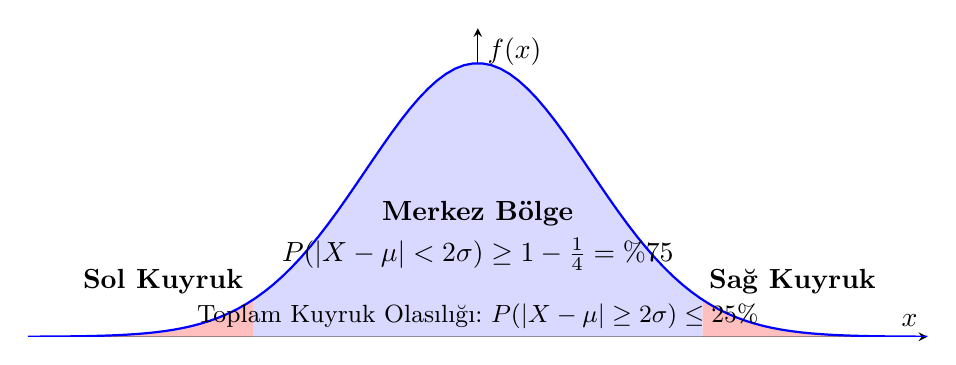
\begin{tikzpicture}
\begin{axis}[
    width=13cm, height=5.5cm,
    axis lines=center,
    xlabel={$x$}, ylabel={$f(x)$},
    xmin=-4, xmax=4,
    ymin=0, ymax=0.45,
    ticks=none,
    samples=100,
    domain=-4:4
]
    % Ortadaki güvenli bölge [-2, 2]
    \addplot[fill=blue!15, draw=none, domain=-2:2] {1/sqrt(2*pi)*exp(-x^2/2)} \closedcycle;
    % Sol kuyruk
    \addplot[fill=red!25, draw=none, domain=-4:-2] {1/sqrt(2*pi)*exp(-x^2/2)} \closedcycle;
    % Sağ kuyruk
    \addplot[fill=red!25, draw=none, domain=2:4] {1/sqrt(2*pi)*exp(-x^2/2)} \closedcycle;

    \addplot[blue, thick] {1/sqrt(2*pi)*exp(-x^2/2)};

    \node at (axis cs:0, 0.18) {\textbf{Merkez Bölge}};
    \node at (axis cs:0, 0.12) {$P(|X-\mu| < 2\sigma) \ge 1 - \frac{1}{4} = \%75$};
    
    \node at (axis cs:-2.8, 0.08) {\textbf{Sol Kuyruk}};
    \node at (axis cs:2.8, 0.08) {\textbf{Sağ Kuyruk}};
    \node at (axis cs:0, 0.03) {\small Toplam Kuyruk Olasılığı: $P(|X-\mu| \ge 2\sigma) \le 25\%$};
\end{axis}
\end{tikzpicture}
\captionof{figure}{Chebyshev Eşitsizliği: Dağılımın şekli ne olursa olsun verilerin en az $\%75$'i $\mu \pm 2\sigma$ aralığında, en az $\%88.9$'u $\mu \pm 3\sigma$ aralığında bulunmak zorundadır.}
\end{center}

\subsection{3. Jensen Eşitsizliği}
\begin{teorem}{Jensen Eşitsizliği}
$g(x)$ dışbükey (convex, yani $g''(x) \ge 0$) bir fonksiyon ve $X$ beklenen değeri sonlu bir rastgele değişken olsun. Bu durumda:
\begin{equation}
    E[g(X)] \ge g(E[X])
\end{equation}
Eğer $g(x)$ içbükey (concave, yani $g''(x) \le 0$) ise eşitsizlik yön değiştirir: $E[g(X)] \le g(E[X])$.
\end{teorem}

\begin{sezgi}{Jensen Eşitsizliği Neden Doğrudur? (Teğet Doğrusu İspatı)}
Dışbükey bir fonksiyonun (örneğin $g(x) = x^2$ veya $g(x) = e^x$) grafiği her zaman herhangi bir noktasından çizilen teğet doğrusunun \textbf{üzerinde kalır}.  
Fonksiyona tam $\mu = E(X)$ noktasından teğet çizelim. Teğet doğrusunun denklemi $L(x) = g(\mu) + g'(\mu)(x - \mu)$'dir.  
Dışbükeylik nedeniyle her $x$ için $g(x) \ge L(x)$ olur:
\begin{equation}
    g(X) \ge g(\mu) + g'(\mu)(X - \mu)
\end{equation}
Her iki tarafın beklenen değerini alırsak:
\begin{equation}
    E[g(X)] \ge g(\mu) + g'(\mu) \underbrace{E(X - \mu)}_{0} = g(\mu) = g(E[X])
\end{equation}
İşte bu kadar zarif bir geometrik gerçek!
\end{sezgi}

\begin{center}
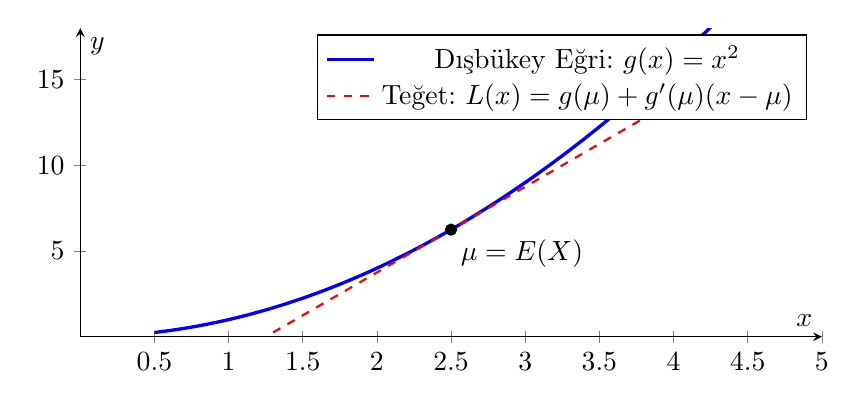
\begin{tikzpicture}
\begin{axis}[
    width=11cm, height=5.5cm,
    axis lines=center,
    xlabel={$x$}, ylabel={$y$},
    xmin=0, xmax=5,
    ymin=0, ymax=18,
    domain=0.5:4.5,
    samples=100
]
    % Dışbükey fonksiyon g(x) = x^2
    \addplot[blue, very thick] {x^2};
    \addlegendentry{Dışbükey Eğri: $g(x) = x^2$}

    % mu = 2.5 noktasındaki teğet: g(2.5)=6.25, g'(2.5)=5 -> y = 6.25 + 5(x - 2.5) = 5x - 6.25
    \addplot[red, thick, dashed, domain=1.3:4.5] {5*x - 6.25};
    \addlegendentry{Teğet: $L(x) = g(\mu) + g'(\mu)(x-\mu)$}

    \draw[fill=black] (axis cs:2.5, 6.25) circle (2pt) node[below right] {$\mu = E(X)$};
    \node[above left] at (axis cs:3.5, 12.25) {$g(x) \ge L(x)$};
\end{axis}
\end{tikzpicture}
\captionof{figure}{Jensen Eşitsizliği Geometrisi: Dışbükey eğri daima teğetinin üstünde kaldığından ortalama değerin fonksiyonu $g(E[X])$, fonksiyonun ortalaması $E[g(X)]$'ten küçük veya eşittir.}
\end{center}

\textbf{Jensen Eşitsizliğinin Doğrudan Sonuçları:}
\begin{enumerate}
    \item $g(x) = x^2$ dışbükeydir $\implies E(X^2) \ge [E(X)]^2 \iff V(X) = E(X^2) - [E(X)]^2 \ge 0$. (Varyansın negatif olamayacağının en temel ispatı!)
    \item $g(x) = 1/x$ ($x > 0$ için dışbükey) $\implies E\left(\frac{1}{X}\right) \ge \frac{1}{E(X)}$.
    \item $g(x) = -\ln(x)$ dışbükey $\implies E[\ln X] \le \ln(E[X])$. (Aritmetik Ortalama $\ge$ Geometrik Ortalama eşitsizliğinin temeli).
\end{enumerate}

---

\section{Moment Çıkaran Fonksiyon (MÇF / MGF)}

\begin{sezgi}{Neden MÇF? (Türevle Moment Üreten Tohum Fonksiyon)}
Her bir $k$. moment için ayrı ayrı zorlu integraller ($\int x^k f(x) dx$) çözmek yerine, bütün momentleri bünyesinde bir katsayı olarak saklayan fonksiyon:
\begin{equation}
    M_X(t) = E(e^{tX})
\end{equation}
şeklinde tanımlanır. Bu fonksiyondan $t$'ye göre $k$ kez türev alıp $t=0$ koyduğumuzda doğrudan $k$. moment önümüze düşer.
\end{sezgi}

\begin{tanim}{Moment Çıkaran Fonksiyon Tanımı}
Bir $X$ rastgele değişkeni için moment çıkaran fonksiyon $M_X(t)$ şu şekilde tanımlanır:
\begin{equation}
    M_X(t) = E(e^{tX}) = 
    \begin{cases}
        \sum_x e^{tx} P(X = x), & \text{kesikli durumda} \\[0.5em]
        \int_{-\infty}^{\infty} e^{tx} f(x) \, dx, & \text{sürekli durumda}
    \end{cases}
\end{equation}
\textit{Varlık Koşulu:} $M_X(t)$'nin var olması için $0$ civarında en az bir $(-h, h)$ aralığında ($h > 0$) bu beklenen değerin sonlu olması şarttır.
\end{tanim}

\subsection{Moment Çıkaran Fonksiyonun Temel Özellikleri}
\begin{enumerate}
    \item \textbf{Sıfır Noktasındaki Değer:}
    \begin{equation}
        M_X(0) = E(e^{0 \cdot X}) = E(1) = 1
    \end{equation}
    Bu özellik MÇF türetimlerinde sağlama yapmak için harika bir kontrol aracıdır.

    \item \textbf{Momentleri Türetme Mekanizması:}
    $e^u = \sum_{k=0}^\infty \frac{u^k}{k!}$ Maclaurin seri açılımından:
    \begin{equation}
        M_X(t) = E\left[ \sum_{k=0}^\infty \frac{(tX)^k}{k!} \right] = \sum_{k=0}^\infty \frac{t^k}{k!} E(X^k) = 1 + t E(X) + \frac{t^2}{2!} E(X^2) + \dots + \frac{t^k}{k!} E(X^k) + \dots
    \end{equation}
    Dolayısıyla $t$'ye göre $k$. türev alınıp $t=0$ yazıldığında:
    \begin{equation}
        \left. \frac{d^k M_X(t)}{dt^k} \right|_{t=0} = E(X^k) = \mu'_k
    \end{equation}

    \item \textbf{Doğrusal Dönüşüm Kuralı:}
    Eğer $Y = aX + b$ ise ($a, b \in \mathbb{R}$):
    \begin{equation}
        M_Y(t) = E(e^{t(aX+b)}) = E(e^{bt} e^{(at)X}) = e^{bt} E(e^{(at)X}) = e^{bt} M_X(at)
    \end{equation}

    \item \textbf{Teklik Teoremi (Uniqueness Theorem):}
    Eğer iki rastgele değişkenin bir $(-h, h)$ aralığında MÇF'leri eşitse ($M_X(t) = M_Y(t)$), bu iki değişkenin kitle olasılık dağılımları birebir aynıdır ($F_X(x) = F_Y(x)$). MÇF bir dağılımın genetik parmak izidir.
\end{enumerate}

\begin{ornek}{Standart Normal $N(0,1)$ ve Genel Normal $N(\mu, \sigma^2)$ MÇF'si}
\textbf{Adım 1: Standart Normal $Z \sim N(0,1)$ için:}
\begin{align}
    M_Z(t) &= E(e^{tZ}) = \int_{-\infty}^{\infty} e^{tz} \frac{1}{\sqrt{2\pi}} e^{-\frac{z^2}{2}} dz = \frac{1}{\sqrt{2\pi}} \int_{-\infty}^{\infty} e^{-\frac{1}{2}(z^2 - 2tz)} dz \notag \\
    &= \frac{1}{\sqrt{2\pi}} \int_{-\infty}^{\infty} e^{-\frac{1}{2}[(z-t)^2 - t^2]} dz = e^{\frac{t^2}{2}} \underbrace{\int_{-\infty}^{\infty} \frac{1}{\sqrt{2\pi}} e^{-\frac{(z-t)^2}{2}} dz}_{1} = e^{\frac{t^2}{2}}
\end{align}

\textbf{Adım 2: Genel Normal $X = \sigma Z + \mu \sim N(\mu, \sigma^2)$ için Doğrusal Dönüşümle:}  
Doğrusal dönüşüm kuralı $M_{aZ+b}(t) = e^{bt} M_Z(at)$ kullanılarak integral çözmeden anında:
\begin{equation}
    \boxed{M_X(t) = e^{\mu t} M_Z(\sigma t) = e^{\mu t} e^{\frac{(\sigma t)^2}{2}} = \exp\left( \mu t + \frac{1}{2}\sigma^2 t^2 \right)}
\end{equation}
bulunur.
\end{ornek}

\subsection{Kümülan Çıkaran Fonksiyon (Cumulant Generating Function)}
MÇF'nin doğal logaritması \textbf{Kümülan Çıkaran Fonksiyon} olarak adlandırılır:
\begin{equation}
    K_X(t) = \ln M_X(t)
\end{equation}
Bu fonksiyon özellikle varyans ve yüksek momentlerin hesabında türev işlemlerini olağanüstü kolaylaştırır:
\begin{align}
    K'_X(t) &= \frac{M'_X(t)}{M_X(t)} \implies K'_X(0) = \frac{M'_X(0)}{M_X(0)} = \frac{E(X)}{1} = \mu \\
    K''_X(t) &= \frac{M''_X(t) M_X(t) - [M'_X(t)]^2}{[M_X(t)]^2} \implies K''_X(0) = \frac{E(X^2) \cdot 1 - [E(X)]^2}{1^2} = \sigma^2
\end{align}
Normal dağılım için $K_X(t) = \ln\left( e^{\mu t + \frac{1}{2}\sigma^2 t^2} \right) = \mu t + \frac{1}{2}\sigma^2 t^2$ olur.  
Görüldüğü üzere $K'_X(0) = \mu$ ve $K''_X(0) = \sigma^2$ anında çıkar!

---

\section{Bileşik MÇF, Bağımsızlık ve Toplamların Dağılımı}

\begin{tanim}{Bileşik Moment Çıkaran Fonksiyon}
$\underline{X} = (X_1, X_2, \dots, X_n)$ sürekli rastgele değişkenler vektörü ve ortak olasılık yoğunluğu $f(x_1, \dots, x_n)$ olsun:
\begin{equation}
    M_{\underline{X}}(t_1, \dots, t_n) = E\left( e^{t_1 X_1 + \dots + t_n X_n} \right) = \int_{-\infty}^\infty \dots \int_{-\infty}^\infty e^{\sum_{i=1}^n t_i x_i} f(x_1, \dots, x_n) dx_1 \dots dx_n
\end{equation}
\end{tanim}

\subsection{Bağımsızlık Durumu}
Eğer $X_1, \dots, X_n$ rastgele değişkenleri bağımsız ise ortak yoğunluk marjinal yoğunlukların çarpımıdır: $f(x_1,\dots,x_n) = \prod_{i=1}^n f_{X_i}(x_i)$.  
Bu durumda bileşik MÇF, marjinal MÇF'lerin basit bir çarpımına ayrışır:
\begin{equation}
    M_{\underline{X}}(t_1, \dots, t_n) = \prod_{i=1}^n M_{X_i}(t_i)
\end{equation}

\subsection{Bağımsız Değişkenlerin Toplamı}
\begin{teorem}{Toplamın MÇF Teoremi}
$X_1, X_2, \dots, X_n$ karşılıklı bağımsız rastgele değişkenler ve toplamları $Y = \sum_{i=1}^n X_i$ olsun:
\begin{equation}
    M_Y(t) = E(e^{tY}) = E\left(e^{t \sum X_i}\right) = E\left( \prod_{i=1}^n e^{t X_i} \right) = \prod_{i=1}^n E(e^{t X_i}) = \prod_{i=1}^n M_{X_i}(t)
\end{equation}
Eğer bu değişkenler bağımsız ve özdeş dağılımlı (i.i.d.) ise:
\begin{equation}
    M_Y(t) = \left[ M_X(t) \right]^n
\end{equation}
\end{teorem}

\begin{ornek}{Bağımsız Poisson Değişkenlerinin Toplamı}
$X_1 \sim \text{Poisson}(\lambda_1)$ ve $X_2 \sim \text{Poisson}(\lambda_2)$ bağımsız olsun. $Y = X_1 + X_2$'nin dağılımını MÇF yöntemiyle bulunuz.

\bigskip
\textbf{Çözüm:}
\begin{enumerate}
    \item Tek bir Poisson($\lambda$) değişkeninin MÇF'si:
    \begin{align}
        M_X(t) &= E(e^{tX}) = \sum_{x=0}^\infty e^{tx} \frac{e^{-\lambda}\lambda^x}{x!} = e^{-\lambda} \sum_{x=0}^\infty \frac{(\lambda e^t)^x}{x!} \notag \\
        &= e^{-\lambda} e^{\lambda e^t} = \exp\left( \lambda(e^t - 1) \right)
    \end{align}
    \item Bağımsız toplamın MÇF'si:
    \begin{align}
        M_Y(t) &= M_{X_1}(t) \cdot M_{X_2}(t) = \exp\left(\lambda_1(e^t - 1)\right) \cdot \exp\left(\lambda_2(e^t - 1)\right) \notag \\
        &= \exp\left( (\lambda_1 + \lambda_2)(e^t - 1) \right)
    \end{align}
    \item \textbf{Teklik Teoremi:} Bu ifade parametresi $(\lambda_1 + \lambda_2)$ olan bir Poisson MÇF'sidir. Dolayısıyla:
    \begin{equation}
        \boxed{X_1 + X_2 \sim \text{Poisson}(\lambda_1 + \lambda_2)}
    \end{equation}
\end{enumerate}
\end{ornek}

\begin{ornek}{Üstel Dağılımlı Değişkenlerin Toplamı ve Gamma Dağılımı}
$X_1, \dots, X_n \overset{\text{i.i.d.}}{\sim} \text{Üstel}(\lambda)$ olsun: $f(x) = \lambda e^{-\lambda x}, \; x > 0$. $Y = \sum_{i=1}^n X_i$'nin dağılımını belirleyiniz.

\bigskip
\textbf{Çözüm:}
\begin{enumerate}
    \item Tek bir üstel değişkenin MÇF'si:
    \begin{equation}
        M_X(t) = \int_0^\infty e^{tx} \lambda e^{-\lambda x} dx = \lambda \int_0^\infty e^{-(\lambda - t)x} dx = \frac{\lambda}{\lambda - t} = \left( 1 - \frac{t}{\lambda} \right)^{-1}, \quad (t < \lambda)
    \end{equation}
    \item $n$ bağımsız değişkenin toplamı için:
    \begin{equation}
        M_Y(t) = [M_X(t)]^n = \left( 1 - \frac{t}{\lambda} \right)^{-n} = \left( \frac{\lambda}{\lambda - t} \right)^n
    \end{equation}
    \item Bu formül şekil parametresi $n$ ve oran parametresi $\lambda$ olan \textbf{Gamma Dağılımı}'nın MÇF'sidir:
    \begin{equation}
        \boxed{Y = \sum_{i=1}^n X_i \sim \text{Gamma}(n, \lambda)}
    \end{equation}
\end{enumerate}
\end{ornek}

\begin{center}
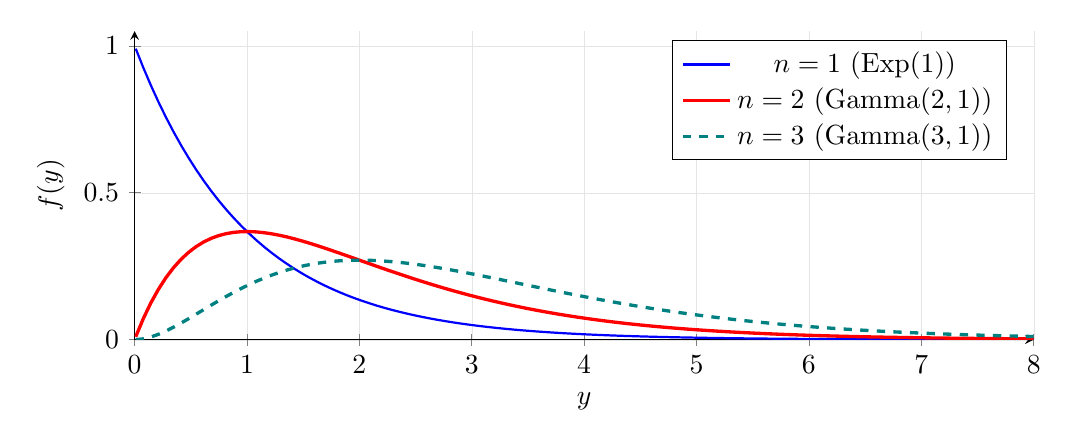
\begin{tikzpicture}
\begin{axis}[
    width=13cm, height=5.5cm,
    axis lines=left,
    xlabel={$y$}, ylabel={$f(y)$},
    xmin=0, xmax=8,
    ymin=0, ymax=1.05,
    samples=120,
    domain=0.01:8,
    legend pos=north east,
    grid=both,
    grid style={line width=.1pt, draw=gray!20}
]
    \addplot[blue, thick] {exp(-x)};
    \addlegendentry{$n=1$ ($\text{Exp}(1)$)}

    \addplot[red, very thick] {x * exp(-x)};
    \addlegendentry{$n=2$ ($\text{Gamma}(2, 1)$)}

    \addplot[teal, very thick, dashed] {0.5 * x^2 * exp(-x)};
    \addlegendentry{$n=3$ ($\text{Gamma}(3, 1)$)}
\end{axis}
\end{tikzpicture}
\captionof{figure}{Bağımsız $n$ adet $\text{Exp}(1)$ değişkeninin toplamı $\text{Gamma}(n, 1)$ dağılımına dönüşür. $n$ büyüdükçe tepe noktası sağa kayar ve çan eğrisine simetrikleşir.}
\end{center}

---

\section{Gamma Fonksiyonu ve Euler İntegrali}

\begin{sezgi}{Gamma Fonksiyonu Nedir?}
Gamma fonksiyonu, faktöriyel kavramının tam sayılardan tüm pozitif reel ve karmaşık sayılara genelleştirilmiş halidir:
\begin{itemize}
    \item Pozitif tam sayılar için: $\Gamma(n) = (n-1)!$ (Örn: $\Gamma(4) = 3! = 6$, $\Gamma(1) = 0! = 1$).
    \item Peki kesirli bir sayının faktöriyeli nedir? Örneğin $\Gamma(1/2) = \sqrt{\pi}$ çıkar. Bu $\sqrt{\pi}$ sabiti, normal dağılımın ve Ki-Kare dağılımlarının kalbindeki temel normalize edicidir.
\end{itemize}
\end{sezgi}

Euler Gamma fonksiyonu şu integral ile tanımlanır:
\begin{equation}
    \Gamma(\alpha) = \int_{0}^{\infty} x^{\alpha - 1} e^{-x} \, dx, \quad (\alpha > 0)
\end{equation}
Ölçek parametresi $\lambda$ eklendiğinde genel Gamma integrali elde edilir:
\begin{equation}
    \int_{0}^{\infty} x^{\alpha - 1} e^{-\lambda x} \, dx = \frac{\Gamma(\alpha)}{\lambda^\alpha}
\end{equation}

\begin{uyari}
\textbf{El Yazısı Notlardaki Çok Önemli Hata ve Doğrusu (Sayfa 5):}
\begin{itemize}
    \item \textbf{Notta Yazılan İfade:} $\Gamma(n) = n \, \Gamma(n-1)$ \textbf{\textcolor{alertred}{(HATALI!)}}
    \item \textbf{Matematiksel Gerçek:} 
    \begin{equation}
        \boxed{\Gamma(n) = (n-1)\Gamma(n-1)} \quad \text{veya} \quad \boxed{\Gamma(n+1) = n\Gamma(n)}
    \end{equation}
    \item \textbf{Neden Hatalı?}  
    Kısmi integrasyon uygulandığında:
    \begin{align}
        \Gamma(n) &= \int_0^\infty x^{n-1} e^{-x} dx \quad \left(u = x^{n-1} \implies du = (n-1)x^{n-2}dx, \; dv = e^{-x}dx \implies v = -e^{-x}\right) \notag \\
        &= \underbrace{\left[ -x^{n-1} e^{-x} \right]_0^\infty}_{0} + (n-1) \int_0^\infty x^{n-2} e^{-x} dx = (n-1)\Gamma(n-1)
    \end{align}
    Nitekim notun hemen altındaki tam sayılarda $\Gamma(n) = (n-1)!$ eşitliği ancak $\Gamma(n) = (n-1)\Gamma(n-1)$ indirgemesiyle tutarlıdır.
\end{itemize}
\end{uyari}

\subsection{Kesirli Değerlerin Hesaplanması}
Yineleme bağıntısı $\Gamma(\alpha+1) = \alpha \Gamma(\alpha)$ kullanılarak:
\begin{align}
    \Gamma\left(\frac{3}{2}\right) &= \frac{1}{2} \Gamma\left(\frac{1}{2}\right) = \frac{\sqrt{\pi}}{2} \\
    \Gamma\left(\frac{5}{2}\right) &= \frac{3}{2} \Gamma\left(\frac{3}{2}\right) = \frac{3}{2} \cdot \frac{\sqrt{\pi}}{2} = \frac{3\sqrt{\pi}}{4} \\
    \Gamma\left(\frac{7}{2}\right) &= \frac{5}{2} \Gamma\left(\frac{5}{2}\right) = \frac{15\sqrt{\pi}}{8}
\end{align}

---

\section{Haftalık Ödev ve 2 Farklı Yoldan Detaylı Çözümü}

\begin{odev}{$\Gamma\left(\frac{1}{2}\right) = \sqrt{\pi}$ Eşitliğinin Gösterilmesi}
\textbf{Problem:} $\Gamma\left(\frac{1}{2}\right) = \sqrt{\pi}$ olduğunu gösteriniz.

\bigskip
\textbf{1. Yöntem (Ders Notundaki İpucu: Standart Normal Dağılım Yardımıyla):}  
Standart normal yoğunluğun simetrisi gereği:
\begin{equation}
    \int_{0}^{\infty} \frac{1}{\sqrt{2\pi}} e^{-\frac{x^2}{2}} dx = \frac{1}{2}
\end{equation}
$u = \frac{x^2}{2}$ değişken dönüşümü yapalım:
\begin{equation}
    x = \sqrt{2} u^{1/2} \implies dx = \frac{\sqrt{2}}{2} u^{-1/2} du = \frac{1}{\sqrt{2}} u^{-1/2} du
\end{equation}
İntegrale yerleştirelim:
\begin{align}
    \int_{0}^{\infty} \frac{1}{\sqrt{2\pi}} e^{-u} \left( \frac{1}{\sqrt{2}} u^{-1/2} du \right) &= \frac{1}{2} \notag \\
    \frac{1}{2\sqrt{\pi}} \int_{0}^{\infty} u^{\frac{1}{2} - 1} e^{-u} du &= \frac{1}{2} \notag \\
    \frac{1}{\sqrt{\pi}} \Gamma\left(\frac{1}{2}\right) = 1 &\implies \boxed{\Gamma\left(\frac{1}{2}\right) = \sqrt{\pi}}
\end{align}

\bigskip
\textbf{2. Yöntem (Kutupsal Koordinatlarla Çift Katlı İntegral Yolu):}  
Tanımdan: $\Gamma(1/2) = \int_0^\infty t^{-1/2} e^{-t} dt$. $t = y^2 \implies dt = 2y \, dy$ dönüşümüyle:
\begin{equation}
    \Gamma\left(\frac{1}{2}\right) = 2 \int_0^\infty e^{-y^2} dy
\end{equation}
Aynı integrali $x$ değişkeniyle çarpalım:
\begin{equation}
    \left[ \Gamma\left(\frac{1}{2}\right) \right]^2 = \left( 2 \int_0^\infty e^{-x^2} dx \right) \left( 2 \int_0^\infty e^{-y^2} dy \right) = 4 \int_0^\infty \int_0^\infty e^{-(x^2 + y^2)} dx \, dy
\end{equation}
1. bölgede kutupsal koordinatlara ($x = r\cos\theta, y = r\sin\theta, dx dy = r dr d\theta, r \in [0, \infty), \theta \in [0, \pi/2]$) geçelim:
\begin{equation}
    \left[ \Gamma\left(\frac{1}{2}\right) \right]^2 = 4 \left( \int_0^{\pi/2} d\theta \right) \left( \int_0^\infty r e^{-r^2} dr \right) = 4 \left( \frac{\pi}{2} \right) \left[ -\frac{1}{2} e^{-r^2} \right]_0^\infty = 2\pi \left(\frac{1}{2}\right) = \pi
\end{equation}
Karekök alındığında:
\begin{equation}
    \boxed{\Gamma\left(\frac{1}{2}\right) = \sqrt{\pi}}
\end{equation}
elde edilir.
\end{odev}

\begin{center}
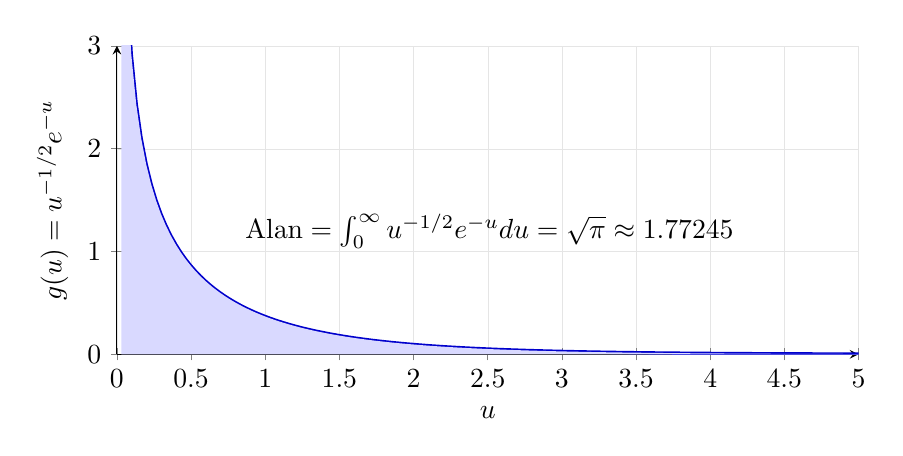
\begin{tikzpicture}
\begin{axis}[
    width=11cm, height=5.5cm,
    axis lines=left,
    xlabel={$u$}, ylabel={$g(u) = u^{-1/2} e^{-u}$},
    xmin=0, xmax=5,
    ymin=0, ymax=3,
    samples=150,
    domain=0.03:5,
    grid=both,
    grid style={line width=.1pt, draw=gray!20}
]
    \addplot[blue!80!black, very thick] {x^(-0.5) * exp(-x)};
    \addplot[fill=blue!15, draw=none, domain=0.03:5] {x^(-0.5) * exp(-x)} \closedcycle;
    \node[right] at (axis cs:0.8, 1.2) {$\text{Alan} = \int_0^\infty u^{-1/2}e^{-u}du = \sqrt{\pi} \approx 1.77245$};
\end{axis}
\end{tikzpicture}
\captionof{figure}{$\Gamma(1/2)$ integrandı: $u \to 0^+$ iken fonksiyon sonsuza ıraksasa da integral yakınsaktır ve toplam alanı tam olarak $\sqrt{\pi}$ değerine eşittir.}
\end{center}

---

\section{1. Hafta Hızlı Tekrar ve Karşılaştırma Kartı}

\begin{table}[ht]
\centering
\small
\renewcommand{\arraystretch}{1.4}
\begin{tabularx}{\textwidth}{@{}l l X@{}}
\toprule
\textbf{Kavram / Teorem} & \textbf{Matematiksel Formül} & \textbf{Sezgisel Anlamı / Ne İşe Yarar?} \\ \midrule
1. Ham Moment & $\mu'_1 = E(X)$ & Dağılımın sayı doğrusundaki ağırlık merkezi (Ortalama) \\
2. Merkezsel Moment & $\mu_2 = E[(X-\mu)^2] = \sigma^2$ & Ağırlık merkezinden saçılma ve belirsizlik ölçüsü (Varyans) \\
Markov Eşitsizliği & $P(X \ge a) \le \frac{E(X)}{a}$ ($X \ge 0$) & Sadece ortalamayı bilerek kuyruk olasılığına evrensel üst sınır \\
Chebyshev Eşitsizliği & $P(|X - \mu| \ge k\sigma) \le \frac{1}{k^2}$ & Şekil ne olursa olsun verilerin $\ge \%75$'i $\mu \pm 2\sigma$ içindedir \\
Jensen Eşitsizliği & $E[g(X)] \ge g(E[X])$ ($g'' \ge 0$) & Dışbükey fonksiyonların beklenen değeri, beklenen değerin fonksiyonundan büyüktür \\
MÇF Tanımı & $M_X(t) = E(e^{tX})$ & Bütün momentleri türev katsayısı olarak saklayan tohum fonksiyon \\
$k$. Moment Çıkarma & $E(X^k) = \left. \frac{d^k M_X(t)}{dt^k} \right|_{t=0}$ & İntegralsiz, yalnızca $k$ kez türev alarak moment bulma \\
Doğrusal Dönüşüm & $M_{aX+b}(t) = e^{bt} M_X(at)$ & Değişken ölçeklendiğinde ve kaydırıldığında MÇF'nin davranışı \\
Bağımsız Toplam & $M_{\sum X_i}(t) = \prod M_{X_i}(t)$ & Zor konvolüsyon integrallerini basit çarpmaya dönüştürür \\
Teklik Teoremi & $M_X(t) = M_Y(t) \implies F_X = F_Y$ & MÇF dağılımın genetik parmak izidir; tek bir dağılımı temsil eder \\
Gamma İndirgeme & $\Gamma(n) = (n-1)\Gamma(n-1)$ & Faktöriyelin reel genellemesi: Tam sayılarda $\Gamma(n) = (n-1)!$ \\
Kritik Özel Değer & $\Gamma(1/2) = \sqrt{\pi}$ & Normal ve Ki-Kare dağılımlarının temel normalize edici sabiti \\ \bottomrule
\end{tabularx}
\caption{1. Haftanın Temel Formül ve Teorem Referans Kartı}
\end{table}

\end{document}
